\documentclass[conference]{IEEEtran}
\IEEEoverridecommandlockouts

\usepackage{cite}
\usepackage{amsmath,amssymb,amsfonts}
\usepackage{algorithmic}
\usepackage{graphicx}
\usepackage{textcomp}
\usepackage{xcolor}
\usepackage{booktabs}
\usepackage{multirow}
\usepackage{array}
\usepackage{url}
\usepackage{tabularx}
\usepackage{tikz}
\usetikzlibrary{arrows.meta,positioning,shapes.geometric,calc}

\def\BibTeX{{\rm B\kern-.05em{\sc i\kern-.025em b}\kern-.08em
    T\kern-.1667em\lower.7ex\hbox{E}\kern-.125emX}}

\begin{document}

\title{Rice Harvest-Readiness Detection on Low-Cost ESP32-CAM IoT: A Comparative Study of ML, DL, Hybrid, and Vision-Language Models}

\author{\IEEEauthorblockN{Ezra Satria Bagas Airlangga}
\IEEEauthorblockA{\textit{School of Electrical Engineering} \\
\textit{Telkom University}\\
Bandung, Indonesia \\
ezrasatriabagas@student.telkomuniversity.ac.id}
\and
\IEEEauthorblockN{Rendy Munadi}
\IEEEauthorblockA{\textit{School of Electrical Engineering} \\
\textit{Telkom University}\\
Bandung, Indonesia \\
rendymunadi@telkomuniversity.ac.id}
\and
\IEEEauthorblockN{Helni Mutiarsih Jumhur}
\IEEEauthorblockA{\textit{School of Electrical Engineering} \\
\textit{Telkom University}\\
Bandung, Indonesia \\
helnimj@telkomuniversity.ac.id}
}

\maketitle

\begin{abstract}
Smallholder rice farmers in Indonesia still rely on subjective visual judgment for harvest timing, while satellite and unmanned-aerial-vehicle remote sensing remain unaffordable at sub-hectare scale, and conventional supervised classifiers force a phenology label on every input under a closed-world assumption. This work develops a low-cost cloud-based pipeline that captures top-down rice canopy images with an ESP32-CAM AI-Thinker module (OV3660 sensor), uploads them through signed URLs to Google Cloud Storage in the Jakarta region, performs inference on a Flask service hosted on Google Cloud Run, and serves predictions to a Progressive Web App dashboard via Firebase Realtime Database. Four classifier families are compared on the same 1140-image curated dataset (1036 cross-validation pool, 104 held-out test) covering vegetative, generative, and mature classes: forty classical configurations of five algorithms over eight color vegetation indices with Gray Level Co-occurrence Matrix texture, three transfer-learned convolutional backbones, three late-fusion hybrid configurations, and four hosted vision-language endpoints used as open-world gatekeepers rather than primary classifiers. The hybrid EfficientNetB0 with ExGR features leads test Macro F1 at 0.9662, while the classical Support Vector Machine with ExGR follows at 0.9577 in a 55~KB artifact; bench-scale validation on the deployed ESP32-CAM sensor shows this test-set parity does not carry over, so the pipeline deploys the hybrid classifier despite its larger footprint. The deployed Gemini~2.5 Flash~Lite gatekeeper rejects all twelve non-rice probes (0\% false-accept rate) at a 4.81\% false-reject rate on rice imagery, and end-to-end bench-scale latency is 8.57~s median, comfortably within a ten-minute capture cadence. The architecture encodes data governance through Indonesia-region residency, separated device and farmer identifiers, and least-privilege access aligned with Indonesian Law No.~27 of 2022 on Personal Data Protection, Government Regulation No.~71 of 2019, ISO/IEC~30141:2024, and ITU-T Recommendation Y.2060.
\end{abstract}

\begin{IEEEkeywords}
rice phenology, proximal imaging, ESP32-CAM, vision-language model, open-set recognition, IoT data governance, smallholder agriculture.
\end{IEEEkeywords}

\section{Introduction}
Rice (\textit{Oryza sativa} L.) is the staple food crop for more than half of the global population, with Asia dominating production and consumption \cite{b_mohidem}. In Indonesia, the 2023 Agricultural Census reports that about 62\% of the 27.8 million agricultural land users are smallholders (\textit{petani gurem}) cultivating less than 0.5 hectares, with food crops as the dominant subsector \cite{b_bps}. For these farmers, harvest timing is decisive: harvesting too early lowers yield and increases chalkiness; delayed harvesting in tropical regions reduces the head rice rate and increases shattering losses \cite{b_zhou}.

Smallholders typically schedule harvest from Days After Sowing or visual inspection, which is imprecise because growth-stage duration varies with cultivar and microclimate \cite{b_sanwong}. Precision agriculture has introduced satellite imagery and unmanned-aerial-vehicle multispectral sensing that correlate strongly with crop phenology through indices such as NDVI \cite{b_huang}, but acquisition cost, recurring operating expense, and required expertise place them out of reach for sub-hectare plots \cite{b_boursianis}. A proximal, in-field, low-cost alternative is therefore needed.

Low-cost embedded imaging modules offer a viable pathway. The ESP32-CAM integrates a camera with a Wi-Fi microcontroller at a price point compatible with smallholder deployment \cite{b_elhattab}. Field imagery from consumer-grade sensors, however, exhibits complex backgrounds, variable illumination, and inadvertent capture of non-rice objects \cite{b_tan}, which require a robust validation step before reliable interpretation. Once a usable canopy image is available, the choice of classifier is not obvious: classical machine learning over hand-crafted vegetation indices and Gray Level Co-occurrence Matrix (GLCM) texture is interpretable and cheap, transfer-learning convolutional neural networks (CNNs) achieve high accuracy on crop classification \cite{b_qin}, hybrid late-fusion combines a CNN backbone with an agronomic prior, and modern vision-language models (VLMs) such as the GPT-4o and Gemini families generalize zero-shot across visual tasks \cite{b_zhang}. No systematic head-to-head comparison of the four families on rice harvest-readiness from low-cost in-field imaging is available.

A second concern is open-set behavior. Closed-world supervised classifiers assign every input to one of the predefined classes regardless of relevance, producing confident but spurious predictions on non-rice frames \cite{b_geng}. Recent evidence on VLMs in agricultural visual recognition shows that accuracy and interpretability are strongly shaped by prompt design rather than raw model capacity, which leaves them short of supervised baselines as primary classifiers in the agricultural domain \cite{b_weedvlm}. This motivates a defensive design: the VLM serves as an \textit{open-world gatekeeper} that rejects non-rice or unusable inputs before a supervised classifier is consulted, rather than as the primary phenology decision.

Finally, an Internet-of-Things agricultural platform that transmits, stores, and processes data across telecommunication networks falls under national and international data-governance frameworks. In Indonesia these include Law No.~19 of 2016 on Electronic Information and Transactions \cite{b_uuite}, Government Regulation No.~71 of 2019 on Electronic Systems and Transactions \cite{b_pp71}, and Law No.~27 of 2022 on Personal Data Protection \cite{b_pdp}. International references include ISO/IEC~30141:2024 on IoT reference architecture \cite{b_iso30141} and ITU-T Recommendation Y.2060 \cite{b_y2060}.

This paper contributes (i) a low-cost ESP32-CAM cloud pipeline that delivers proximal canopy imagery to a Cloud Run inference service with a dashboard; (ii) a systematic four-family comparison (40 classical, 3 deep, 3 hybrid, 4 VLM endpoints) on the same 104-image held-out test set with Macro F1 and Mature Recall under paired 1000-resample bootstrap; (iii) an empirical demonstration that the VLM is best assigned as an open-world gatekeeper rather than the primary classifier; and (iv) a deployment whose data-governance posture is encoded into the architecture.

\section{System Architecture}
The proposed system compares four prediction tracks for rice harvest readiness from RGB images captured by an ESP32-CAM AI-Thinker module with an OV3660 sensor mounted overhead at fixed canopy distance. Three phenological classes are used: \textit{Vegetative} covering tillering and stem elongation, \textit{Generative} covering panicle initiation through flowering, and \textit{Mature} covering grain filling through ripeness where harvest is indicated \cite{b_qin}. Capture runs on the edge device while inference, storage, and dashboard reside in the cloud.

Frames are uploaded from the ESP32-CAM through short-lived signed URLs into a Google Cloud Storage bucket in \texttt{asia-southeast2} (Jakarta), classified by a Cloud Run Flask service, and persisted to Firebase Realtime Database for a Netlify-hosted Progressive Web App dashboard \cite{b_elhattab,b_hercog}. Object names follow the pattern \texttt{\{device\_id\}/\{timestamp\}.jpg} so that frames are partitioned by device without embedding farmer identity. A storage trigger emits an event back to Cloud Run which writes a capture record containing only metadata (device identifier, timestamp, blob URI) so the realtime database stays lean for the dashboard subscription.

Vision-language models serve two roles in this architecture: an \textit{open-world gatekeeper} that rejects non-rice frames before supervised inference, and one of the candidate zero-shot classifiers benchmarked against the supervised tracks \cite{b_geng,b_zhang}. The deployed pipeline routes every accepted frame to the supervised classifier. Data governance is encoded into the architecture by separating device identifiers from farmer identifiers across two database trees with distinct access rules, restricting storage to an Indonesia-eligible region, applying short-expiry per-object signed URLs for device writes, and recording every capture-to-prediction transition in Cloud Logging \cite{b_pdp,b_pp71,b_uuite,b_iso30141}.

\begin{figure}[t]
\centering
\resizebox{\columnwidth}{!}{%
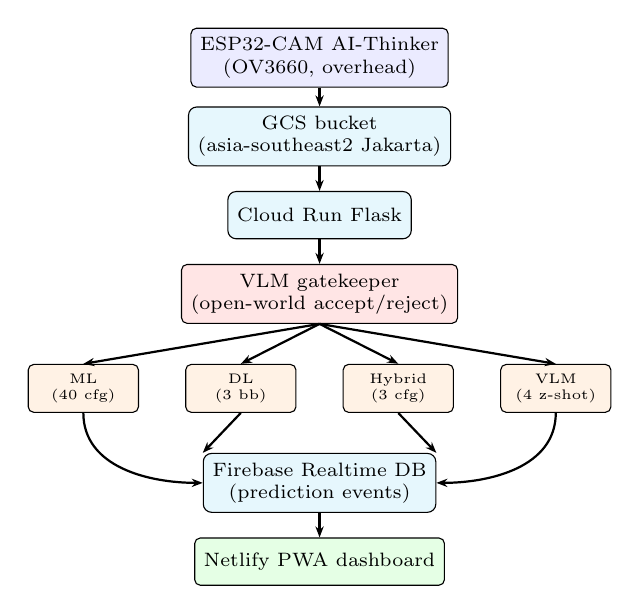
\begin{tikzpicture}[
    edge/.style={draw, rounded corners=2pt, minimum width=22mm, minimum height=6mm, align=center, font=\scriptsize, fill=blue!8},
    cloud/.style={draw, rounded corners=3pt, minimum width=22mm, minimum height=6mm, align=center, font=\scriptsize, fill=cyan!10},
    track/.style={draw, rounded corners=2pt, minimum width=14mm, minimum height=5mm, align=center, font=\tiny, fill=orange!10},
    ui/.style={draw, rounded corners=2pt, minimum width=22mm, minimum height=6mm, align=center, font=\scriptsize, fill=green!10},
    gate/.style={draw, rounded corners=2pt, minimum width=22mm, minimum height=6mm, align=center, font=\scriptsize, fill=red!10},
    arr/.style={-{Stealth[length=1.4mm]}, thick},
]
    \node[edge]  (cam)  at ( 0, 0)    {ESP32-CAM AI-Thinker\\(OV3660, overhead)};
    \node[cloud] (gcs)  at ( 0,-1.0)  {GCS bucket\\(asia-southeast2 Jakarta)};
    \node[cloud] (run)  at ( 0,-2.0)  {Cloud Run Flask};
    \node[gate]  (vlmg) at ( 0,-3.0)  {VLM gatekeeper\\(open-world accept/reject)};
    \node[track] (ml)   at (-3.0,-4.2){ML\\(40 cfg)};
    \node[track] (dl)   at (-1.0,-4.2){DL\\(3 bb)};
    \node[track] (hyb)  at ( 1.0,-4.2){Hybrid\\(3 cfg)};
    \node[track] (vlmc) at ( 3.0,-4.2){VLM\\(4 z-shot)};
    \node[cloud] (rtdb) at ( 0,-5.4)  {Firebase Realtime DB\\(prediction events)};
    \node[ui]    (pwa)  at ( 0,-6.4)  {Netlify PWA dashboard};

    \draw[arr] (cam) -- (gcs);
    \draw[arr] (gcs) -- (run);
    \draw[arr] (run) -- (vlmg);
    \draw[arr] (vlmg.south) -- (ml.north);
    \draw[arr] (vlmg.south) -- (dl.north);
    \draw[arr] (vlmg.south) -- (hyb.north);
    \draw[arr] (vlmg.south) -- (vlmc.north);
    \draw[arr] (ml.south)   to[out=-90,in=180] (rtdb.west);
    \draw[arr] (dl.south)   -- (rtdb.north west);
    \draw[arr] (hyb.south)  -- (rtdb.north east);
    \draw[arr] (vlmc.south) to[out=-90,in=0]   (rtdb.east);
    \draw[arr] (rtdb) -- (pwa);
\end{tikzpicture}%
}
\caption{End-to-end system architecture: ESP32-CAM proximal capture, signed-URL upload to GCS (Jakarta), Cloud Run inference with a VLM gatekeeper preceding the supervised classifier, Firebase Realtime Database, and a Netlify PWA dashboard.}
\label{fig:system}
\end{figure}

\section{Dataset and Preprocessing}
\subsection{Source and Curation}
The training corpus is curated from publicly available RGB rice canopy imagery on Hugging Face (238 images, 45.9\%) and Roboflow Universe (281 images, 54.1\%), totalling 519 raw source images at heterogeneous native resolutions and capture geometries. Aerial frames, sub-canopy close-ups of individual grains, and images with heavy occlusion are removed during curation. A Roboflow processing pipeline resize-fills each frame to $640\times640$, applies contrast stretching, and emits three augmented copies per source training example (horizontal/vertical flip, rotation $\pm15^{\circ}$, brightness $\pm10\%$), expanding the working dataset to 1140 images. The dataset is partitioned once into a 1036-image cross-validation pool (347 Vegetative, 361 Generative, 328 Mature; ratio $1.10$) and a 104-image held-out test set (49/34/21; ratio $2.33$). The same partition is reused across all 46 supervised models and the four VLM endpoints so ranking comparisons are over identical evaluation samples.

\subsection{Preprocessing and Vegetation Indices}
Geometric standardization resizes the shorter side to 224 pixels and center-crops to $224\times224$, matching the native input resolution of EfficientNetB0, MobileNetV2, and MobileNetV3-Small. A tensor path applies ImageNet per-channel normalization for the CNN tracks. A handcrafted path retains a unit-interval RGB array from which eight color vegetation indices are computed (VARI, ExG, ExR, ExGR, GLI, MGRVI, RGBVI, NGRDI) \cite{b_ma}. For each index, ten distributional statistics (mean, standard deviation, median, p10, p25, p75, p90, IQR, and the fractions of pixels above 0 and above 0.1) and eight GLCM features (mean and standard deviation of contrast, homogeneity, energy, and correlation, computed at distances 1 and 3 px and orientations $0^{\circ}, 45^{\circ}, 90^{\circ}, 135^{\circ}$) form an 18-dimensional descriptor per frame \cite{b_liu,b_iqbal}.

\section{Comparative Model Pool}
The supervised pool aggregates three families over the same 1036-image pool and the same 104-image test set, while a fourth track of zero-shot VLMs is evaluated under the identical partition without parameter updates. The configurations are summarized in Table~\ref{tab:pool}.

\begin{table}[t]
\caption{Comparative Pool Summary (46 supervised + 4 zero-shot)}
\label{tab:pool}
\centering
\scriptsize
\setlength{\tabcolsep}{3pt}
\begin{tabular}{@{}l l r@{}}
\toprule
Family & Algorithm / endpoint & Footprint \\
\midrule
Classical & RF, SVM-RBF, KNN, LogReg, GB & 5 algo. \\
Classical & per 8 vegetation indices     & 40 cfg \\
Deep      & EfficientNetB0               & 5.3M, 2-ph TL \\
Deep      & MobileNetV2                  & 3.5M, 2-ph TL \\
Deep      & MobileNetV3-Small            & 2.5M, 2-ph TL \\
Hybrid    & EffNetB0 $\oplus$ ExGR       & 1280+18-d \\
Hybrid    & EffNetB0 $\oplus$ NGRDI      & 1280+18-d \\
Hybrid    & EffNetB0 $\oplus$ VARI       & 1280+18-d \\
VLM       & Gemini 2.5 Flash             & 0 train. \\
VLM       & Gemini 2.5 Flash Lite        & 0 train. \\
VLM       & GPT-4o                       & 0 train. \\
VLM       & GPT-4o mini                  & 0 train. \\
\bottomrule
\end{tabular}
\end{table}

\subsection{Classical, Deep, Hybrid}
Five classical algorithms are evaluated over the 18-dimensional descriptor of each of the eight vegetation indices, yielding a $5\times 8 = 40$-configuration grid: Random Forest, Support Vector Machine with radial basis kernel (SVM-RBF), $k$-Nearest Neighbors, multinomial Logistic Regression, and Gradient Boosting \cite{b_benos,b_suryono}. Three lightweight backbones pretrained on ImageNet are fine-tuned under two-phase transfer learning: EfficientNetB0 (5.3M parameters) \cite{b_efficientnet}, MobileNetV2 (3.5M) \cite{b_mobilenetv2}, and MobileNetV3-Small (2.5M) \cite{b_mobilenetv3}. The hybrid track adopts a late-fusion architecture in which the EfficientNetB0 backbone supplies a 1280-dimensional embedding and the handcrafted pipeline supplies an 18-dimensional descriptor for the same frame, concatenated into a 1298-dimensional vector that feeds a small fully connected head before softmax \cite{b_yang}. Three vegetation indices are paired with the convolutional branch (ExGR, NGRDI, VARI).

\subsection{Vision-Language Track}
Four hosted multimodal endpoints are evaluated under zero-shot prompting on the same test set without rice-specific fine-tuning: Gemini~2.5 Flash, Gemini~2.5 Flash~Lite, GPT-4o, and GPT-4o mini. Each call uses a single structured prompt with temperature 0; the per-call JSON output carries the classification, the confidence score, and an explicit gatekeeper accept flag, so models that decline a frame as out-of-distribution are recorded as rejects rather than as misclassifications.

\subsection{Training Protocol}
The 1036-image pool is partitioned into five class-stratified folds. Fold indices are precomputed once and reused identically across all 46 supervised configurations to keep the ranking paired at the fold level \cite{b_szeghalmy}. Macro F1 is averaged across folds as the cross-validation score; each configuration is then refit on the full pool and evaluated exactly once on the 104-image test set so that the test partition stays decoupled from any tuning decision. Bootstrap 95\% confidence intervals are computed with 1000 paired resamples shared across all 50 evaluated models so that cross-model comparisons remain on the same draws \cite{b_takahashi}.

\section{Results}
\subsection{Cross-Validation}
Table~\ref{tab:cv} summarizes the cross-validation leaders per family. The Hybrid track with NGRDI leads at $0.9770$ Macro F1, the Deep Learning EfficientNetB0 backbone follows at $0.9664$, and the strongest Classical configuration (SVM-RBF with ExGR) reaches $0.9502$.

\begin{table}[t]
\caption{Cross-Validation Leaders per Family (Mean $\pm$ Std)}
\label{tab:cv}
\centering
\begin{tabular}{@{}lll@{}}
\toprule
Family & Configuration & CV Macro F1 \\
\midrule
Hybrid & EffNetB0 + NGRDI & $\mathbf{0.9770 \pm 0.0092}$ \\
Hybrid & EffNetB0 + ExGR  & $0.9691 \pm 0.0089$ \\
Hybrid & EffNetB0 + VARI  & $0.9541 \pm 0.0174$ \\
Deep   & EfficientNetB0   & $0.9664 \pm 0.0086$ \\
Deep   & MobileNetV2      & $0.9270 \pm 0.0170$ \\
Deep   & MobileNetV3-Small & $0.9083 \pm 0.0143$ \\
Classical & SVM(RBF) + ExGR & $0.9502 \pm 0.0070$ \\
Classical & GradBoost + ExGR & $0.9465 \pm 0.0139$ \\
Classical & RF + ExGR        & $0.9418 \pm 0.0141$ \\
\bottomrule
\end{tabular}
\end{table}

\begin{figure}[t]
\centerline{\includegraphics[width=\columnwidth]{fig_cvranking.png}}
\caption{Cross-validation ranking of the 46 supervised models (40 ML + 3 DL + 3 Hybrid) under five-fold stratified CV, error bars show fold standard deviation.}
\label{fig:cvrank}
\end{figure}

\subsection{Held-Out Test Set}
After cross-validation each configuration is refit on the full pool and evaluated once on the 104-image test set. Table~\ref{tab:test} reports the top configuration per supervised track together with Mature Recall, the secondary metric whose false negatives translate into missed harvest timing.

\begin{table}[t]
\caption{Test-set top configurations per track (paired bootstrap 95\% CI, $n=1000$)}
\label{tab:test}
\centering
\footnotesize
\setlength{\tabcolsep}{3pt}
\begin{tabular}{@{}llcc@{}}
\toprule
Track & Configuration & Macro F1 [95\% CI] & Mature Recall \\
\midrule
Hybrid & EffNetB0 + ExGR  & $\mathbf{0.9662}$ [0.92, 1.00] & $0.9553$ \\
Hybrid & EffNetB0 + NGRDI & $0.9621$ [0.91, 1.00] & $0.9553$ \\
ML     & SVM(RBF) + ExGR  & $0.9577$ [0.91, 0.99] & $0.9507$ \\
DL     & EfficientNetB0   & $0.9532$ [0.90, 0.99] & $0.9068$ \\
Hybrid & EffNetB0 + VARI  & $0.9454$ [0.89, 0.99] & $0.9553$ \\
ML     & RF + ExGR        & $0.9368$ [0.88, 0.98] & $0.9030$ \\
DL     & MobileNetV3-Small & $0.9198$ [0.85, 0.97] & $0.8591$ \\
DL     & MobileNetV2      & $0.8821$ [0.81, 0.94] & $0.7656$ \\
\bottomrule
\end{tabular}
\end{table}

The supervised test ranking moves the Hybrid winner from NGRDI (CV) to ExGR (test), leaves EfficientNetB0 in the Deep Learning lead, and keeps SVM-RBF + ExGR as the strongest Classical configuration. Point estimates compress into a narrow band between Macro F1 $0.94$ and $0.97$ for the top of each family, and the bootstrap intervals on the top eight configurations all overlap. The cross-track ordering Hybrid $>$ Classical $>$ Deep is therefore not statistically separable on the held-out sample, which moves the comparative conclusion onto the joint Pareto view together with operational cost (Section \ref{sec:cost}). Fig.~\ref{fig:forest} shows the forest of bootstrap intervals; Fig.~\ref{fig:pareto} shows the joint Macro F1 versus Mature Recall scatter with the Pareto frontier drawn explicitly.

\begin{figure}[t]
\centerline{\includegraphics[width=\columnwidth]{fig_forest.png}}
\caption{Bootstrap 95\% CI forest plot on Macro F1 for the top configurations per track on the 104-image held-out test set.}
\label{fig:forest}
\end{figure}

\begin{figure}[t]
\centerline{\includegraphics[width=\columnwidth]{fig_pareto.png}}
\caption{Joint Pareto frontier: Macro F1 versus Mature Recall for the 50 evaluated models (40 ML + 3 DL + 3 Hybrid + 4 VLM).}
\label{fig:pareto}
\end{figure}

\subsection{Zero-Shot Vision-Language Endpoints}
Table~\ref{tab:vlm} reports the four VLM endpoints under identical prompting on the same 104-image test set. Gemini~2.5 Flash~Lite leads at Macro F1 $0.941$, which is $0.025$ below the supervised Hybrid leader and $0.017$ below the Classical leader.

\begin{table}[t]
\caption{VLM zero-shot results on the 104-image test set}
\label{tab:vlm}
\centering
\footnotesize
\setlength{\tabcolsep}{4pt}
\begin{tabular}{@{}lcccc@{}}
\toprule
Endpoint & Accept & Macro F1 & Mature R. & Acc. \\
\midrule
Gemini 2.5 Flash Lite & 0.952 & $\mathbf{0.941}$ & 1.000 & 0.949 \\
GPT-4o mini           & 1.000 & 0.892 & 0.952 & 0.913 \\
GPT-4o                & 0.990 & 0.831 & 1.000 & 0.864 \\
Gemini 2.5 Flash      & 1.000 & 0.811 & 1.000 & 0.846 \\
\bottomrule
\end{tabular}
\end{table}

The smaller-than-expected zero-shot gap is shaped by a class-specific failure pattern: all four endpoints over-trigger the Mature label on Generative frames at varying severity (Gemini Flash $14/34$, GPT-4o $13/34$, GPT-4o mini $7/34$, Flash Lite $3/31$ of accepted Generative frames), so Macro F1 is reduced by low Generative recall while Mature Recall on accepted samples stays at $0.952$ or above. The pattern is vendor-agnostic, scales inversely with model size, and is consistent with a prompt-bound interpretation of mature canopy cues.

\subsection{Per-Class Diagnostics}
The Classical leader (SVM-RBF + ExGR) misclassifies 4 of 104 test images and yields per-class precision/recall/F1 of $0.98/0.96/0.97$ on Vegetative, $0.94/0.97/0.96$ on Generative, and $0.95/0.95/0.95$ on Mature. The Vegetative--Generative pair carries the most residual confusion, consistent with the canopy color overlap during stem elongation and panicle initiation. Permutation importance with 30 repeats ranks the dispersion of the ExGR signal (\texttt{ExGR\_std}) as the dominant feature at $0.1408 \pm 0.0380$, roughly four times larger than the next feature; four of the top five entries are either ExGR statistics or GLCM descriptors. Fig.~\ref{fig:confusion} shows the confusion matrices for the top model per family.

\begin{figure}[t]
\centerline{\includegraphics[width=\columnwidth]{fig_confusion.png}}
\caption{Confusion matrices for the top configuration per track on the 104-image test set: Classical, Deep, Hybrid, and VLM.}
\label{fig:confusion}
\end{figure}

\subsection{Bench-Scale Field Validation}
A bench-scale rig of four polybag-grown rice plants inside a single litter box with the ESP32-CAM mounted overhead at fixed height is exercised across three scenarios: end-to-end capture-cycle latency, gatekeeper behavior on non-rice probes, and Mature carry-over against the curated test-set Mature Recall. The polybag plants are at the Mature stage for the full duration of validation, so the rice-class measurements are reported for Mature only.

End-to-end latency is recorded at four checkpoints. The deployed pipeline runs Gemini~2.5 Flash~Lite as gatekeeper followed by the Hybrid CNN on a single Cloud Run service in \texttt{asia-southeast2} with 1~vCPU and 512~MiB. Table~\ref{tab:latency} reports the breakdown; the QXGA JPEG is around 200~KB. Server-side compute is dominated by the gatekeeper LLM call ($3865$~ms median), JPEG decode is negligible ($23$~ms), and end-to-end median is $8.57$~s, comfortably within a ten-minute capture cadence. The p95 of $29.88$~s reflects a single Cloud Run cold-start outlier on the first request after scale-from-zero with model load.

\begin{table}[t]
\caption{Bench-scale end-to-end capture cycle latency}
\label{tab:latency}
\centering
\footnotesize
\setlength{\tabcolsep}{4pt}
\begin{tabular}{@{}lrrr@{}}
\toprule
Stage & $n$ & Median (ms) & p95 (ms) \\
\midrule
End-to-end ($T_1 \to T_{resp}$) & 12 & 8570 & 29878 \\
\quad Network + upload (Wi-Fi + TLS) & 12 & 3688 & 10901 \\
Server total ($T_2 \to T_4$)    & 51 & 4006 & 7750 \\
\quad JPEG decode               & 51 & 23   & 36 \\
\quad Gatekeeper LLM + CNN compute & 51 & 3865 & 7592 \\
\quad Response wrap             & 36 & 128  & 164 \\
\midrule
Path: gatekeeper-rejected (LLM only)    & 15 & 4692 & 6488 \\
Path: accepted (LLM + Hybrid CNN)       & 36 & 3868 & 9284 \\
\bottomrule
\end{tabular}
\end{table}

\begin{figure}[t]
\centerline{\includegraphics[width=\columnwidth]{fig_latency.png}}
\caption{Cloud Run server-side latency distribution on the bench-scale rig, accepted vs.\ rejected paths.}
\label{fig:latency}
\end{figure}

The gatekeeper is probed with twelve non-rice frames (four empty-litter-box frames, four with a hand in the field of view, four with a non-rice plant). All four endpoints reject all twelve probes, giving a false-accept rate of $0\%$ across the cohort. False-reject rate on the curated rice test set varies by endpoint: Gemini~2.5 Flash~Lite rejects $5/104 = 4.81\%$ (one Vegetative, three Generative, one Mature), GPT-4o rejects $1/104 = 0.96\%$, and Gemini~2.5 Flash and GPT-4o mini reject none. The deployed pipeline therefore operates at a $4.81\%$ false-reject rate on rice imagery against a $0\%$ false-accept rate on non-rice probes.

Fifty-one ESP32-CAM Mature captures are routed through both supervised leaders and the four-model VLM cohort. The two supervised leaders diverge sharply: Hybrid improves $+4.5$~pp to $1.0000$, while Classical collapses $-95.1$~pp to $0.0000$, misclassifying all $51$ frames ($47$ as Vegetative, $4$ as Generative). The Classical descriptor is computed over the full unmasked frame, so it mixes background and lighting statistics that the tightly-cropped curated training images never carried; the Hybrid classifier avoids this failure mode because its convolutional branch reads the raw image directly instead of relying on the 18-dimensional handcrafted vector alone. A branch-ablation check confirms the descriptor itself is not the point of failure: feeding the Hybrid fusion head the real descriptor with the image branch replaced by a neutral gray frame still classifies all $51$ bench frames as Mature, and the same 18 numbers that the Classical SVM's RBF kernel reads as Vegetative are read correctly by the fusion head trained jointly with the image branch. The VLM cohort splits sharply as well: GPT-4o stays at $1.0000$, Gemini~2.5 Flash loses $-11.8$~pp, Flash~Lite loses $-7.0$~pp, and GPT-4o mini collapses by $-54.1$~pp to $0.4118$ by rejecting $30$ of $51$ bench frames on a stated domain-mismatch reason. Among the VLM cohort the drop scales inversely with model capacity and is consistent with a field-imagery prior present in the smaller endpoints' pretraining distribution.

\subsection{Operational Cost}\label{sec:cost}
Table~\ref{tab:cost} summarizes operational cost across the four tracks. The Classical leader serializes to a $55$~KB joblib file, more than two orders of magnitude smaller than the $\sim$$17$~MB EfficientNetB0 SavedModel used by the Deep and Hybrid leaders; the footprint difference compounds at Cloud Run cold start. With Gemini~2.5 Flash~Lite as gatekeeper and any of the three supervised tracks as classifier, the per-thousand-inference budget is dominated by the synchronous gatekeeper wait and is near US\$$0.12$ per thousand calls. Replacing the gatekeeper with GPT-4o raises the per-call cost by an order of magnitude on the VLM line item. The cost axis therefore favors keeping the cheaper Gemini tier on the gatekeeper side whenever Mature Recall is not the binding constraint.

\begin{table}[t]
\caption{Per-inference cost on the deployed pipeline}
\label{tab:cost}
\centering
\footnotesize
\setlength{\tabcolsep}{3pt}
\begin{tabular}{@{}p{38mm}lr@{}}
\toprule
Track / Endpoint & Artifact & USD / 1k \\
\midrule
Classical: SVM(RBF) + ExGR     & $55$ KB      & $\sim$0.003 \\
DL: EfficientNetB0             & $\sim$17 MB  & $\sim$0.005 \\
Hybrid: EffNetB0 + ExGR        & $\sim$17 MB  & $\sim$0.005 \\
VLM: Gemini 2.5 Flash Lite     & N/A          & $\sim$0.045 \\
VLM: GPT-4o mini               & N/A          & $\sim$0.068 \\
VLM: Gemini 2.5 Flash          & N/A          & $\sim$0.20 \\
VLM: GPT-4o                    & N/A          & $\sim$1.13 \\
\bottomrule
\end{tabular}
\end{table}

\section{Discussion}
\subsection{Hybrid: CV vs.\ Test}
NGRDI leads the cross-validation pool at $0.9770$ but ExGR leads the test set at $0.9662$, a crossover of about $0.005$ between the two hybrid vegetation-index variants. With $n=104$ on the test set and $n=21$ on the Mature subset, the bootstrap intervals overlap substantially and the crossover does not falsify the cross-validation ranking. The methodological take-away is that paired bootstrap intervals, not point-estimate ordinals, are the right object to compare.

\subsection{SVM-RBF as a Cheap Baseline}
SVM-RBF + ExGR reaches $0.9577$ Macro F1, $0.0085$ below the Hybrid leader and $0.0045$ above the Deep Learning backbone, while operating on an 18-dimensional descriptor instead of a 1280-dimensional EfficientNetB0 embedding. The serialized model is on the order of one megabyte versus tens of megabytes for the EfficientNetB0-based pipeline, and inference is a single kernel evaluation rather than a CNN forward pass \cite{b_efficientnet,b_mobilenetv2}. On the curated test set this looks like a favorable trade: a tiny Macro F1 deficit for a meaningfully smaller cold-start footprint. That trade does not survive contact with the deployment sensor: on the ESP32-CAM bench set the Classical configuration collapses to $0.0000$ Mature Recall while Hybrid reaches $1.0000$ on the same frames. The footprint advantage is real, but it does not substitute for the raw-image branch that lets Hybrid generalize past the curated dataset's crop and lighting conditions.

\subsection{VLM Gap and Gatekeeper Role}
The zero-shot VLM endpoints are not exposed to rice-stage supervision, so a Macro F1 deficit relative to the supervised pool is expected, and the open-set classification literature reports similar narrow-domain zero-shot gaps on agricultural imagery \cite{b_geng,b_zhang,b_weedvlm}. The deficit observed here is narrower than expected at $0.025$ Macro F1, but two findings keep the VLM family out of the primary classifier role. First, Generative is systematically over-classified as Mature across all four endpoints, which is a class-pair confusion at the exact transition that the harvest-timing objective is most sensitive to. Second, the bench-scale carry-over result shows that the smaller endpoints drop sharply on ESP32-CAM imagery, with GPT-4o mini collapsing to $0.4118$ Mature Recall against a curated value of $0.9524$, while the supervised Hybrid improves to perfect Mature Recall on the same bench captures. Reassigning the VLM endpoints to the gatekeeper task they natively support yields a $0\%$ false-accept rate on twelve non-rice probes across all four endpoints.

\subsection{Deployment under Governance}\label{sec:discuss-gov}
The deployed pipeline encodes Indonesian data-governance obligations directly into the architecture rather than as a post-hoc compliance exercise: storage residency is constrained to \texttt{asia-southeast2}, device identifiers are separated from farmer identifiers across two Realtime Database trees with distinct access rules, raw frames carry a documented lifecycle window, signed-URL device writes are scoped per object with short expiry, and every capture-to-dashboard transition is captured in Cloud Logging. Table~\ref{tab:gov} maps each regulatory anchor to a concrete architectural artifact and the runtime evidence that supports it, covering Law No.~19 of 2016 \cite{b_uuite}, Government Regulation No.~71 of 2019 \cite{b_pp71}, three provisions of Law No.~27 of 2022 on Personal Data Protection \cite{b_pdp}, ISO/IEC~30141:2024 \cite{b_iso30141}, and ITU-T Recommendation Y.2060 \cite{b_y2060}. The comparative results convert this posture into two operational levers. The first is architectural assignment: the VLM operating as a binary rice-or-not gatekeeper concentrates the cross-border transfer surface to the smallest payload sent to a foreign-hosted endpoint under the third-country transfer provisions of Article~56 of Law No.~27 of 2022. The second is model selection, and here the audit-surface argument only applies to a classifier that works on the deployed sensor: the $55$~KB Classical artifact would reduce the storage and compute surface that downstream audit, retention, and DPIA scoping must cover under Article~20 of Law No.~27 of 2022, but the bench-scale result above shows the Classical configuration fails on ESP32-CAM imagery ($0.0000$ Mature Recall against $1.0000$ for Hybrid), so the deployed pipeline uses the Hybrid classifier regardless of its larger footprint.

\begin{table*}[t]
\caption{Regulatory Crosswalk: Anchor $\to$ Architectural Artifact $\to$ Evidence}
\label{tab:gov}
\scriptsize
\renewcommand{\arraystretch}{1.2}
\setlength{\tabcolsep}{4pt}
\begin{tabularx}{\textwidth}{|>{\raggedright\arraybackslash}p{2.4cm}|>{\raggedright\arraybackslash}X|>{\raggedright\arraybackslash}X|>{\raggedright\arraybackslash}X|}
\hline
\textbf{Source} & \textbf{Obligation} & \textbf{Architectural artifact} & \textbf{Evidence} \\
\hline
Law 19/2016 (ITE) & Integrity and authenticity of electronic information & Signed-URL upload binds each frame to verifiable provenance before inference & Latency log entries trace device, object, and prediction per capture \\
\hline
PP 71/2019 Art.~14 & Operator obligations: purpose limitation, security protection, retention lifecycle, breach notification & Identifier separation (\texttt{device\_id} path, no farmer token in object name), GCS lifecycle-delete rule on raw frames, Cloud Logging for breach traceability & No farmer identifier appears in GCS object names or inference logs; lifecycle policy enforces deletion after retention window \\
\hline
Law 27/2022 Art.~16 (PDP) & Data minimization, purpose limitation & Two separate RTDB trees for device identifiers and farmer identifiers with non-overlapping access rules & No analytical read path joins farmer identity to imagery in the inference logs \\
\hline
Law 27/2022 Art.~20 (PDP) & Controller must document a lawful processing basis & Legitimate-interest basis Art.~20(2)(f) documented; scoped Cloud Run IAM restricts inference to declared agricultural-monitoring purpose & Per-event inference log records device identifier, predicted class, and model version as traceability evidence \\
\hline
Law 27/2022 Art.~56 (PDP) & Third-country transfer minimization & VLM used only as binary rice-or-not gatekeeper, not as classifier & $0\%$ false-accept on 12 non-rice probes; foreign endpoint sees only the smallest decision \\
\hline
ISO/IEC 30141:2024 & Cross-layer data protection (perception, network, application, security) & Scoped writes at perception, TLS at network, gatekeeper + supervised classifier at application, IAM + Cloud Logging at security & Latency budget decomposes across layers ($\sim$3.7~s Wi-Fi, $\sim$4~s warm Cloud Run) \\
\hline
ITU-T Y.2060 & Interconnectivity, autonomic exchange, embedded security & Same scoped-write and structured-log surface as above & $8.57$~s end-to-end median latency under warm-state cycle \\
\hline
\end{tabularx}
\end{table*}

\subsection{Limitations}
The Mature class has support 21 on the test set, so the bootstrap interval on Mature Recall is wide ($[0.85, 1.00]$ for the Classical leader). Bench-scale field validation is restricted to the Mature class on four polybag-grown plants, so Vegetative and Generative performance on ESP32-CAM imagery has not been measured. The VLM results reflect a single prompt design held constant across endpoints, so the systematic Generative-to-Mature confusion and the bench-scale rejection behavior of smaller endpoints could be partially attributable to the prompt rather than the models; a prompt-sensitivity study is left to future work.

\section{Conclusion}
This study has presented a low-cost ESP32-CAM cloud pipeline for rice harvest-readiness detection on smallholder plots, with bench-scale validation on four polybag-grown plants inside a single litter box. A four-family comparison on the same curated 1140-image dataset converges on a tight accuracy band on the held-out test set: the hybrid EfficientNetB0 with ExGR leads at Macro F1 $0.9662$, the classical SVM-RBF with ExGR follows at $0.9577$ in a $55$~KB artifact, and the EfficientNetB0 baseline reaches $0.9532$. Bootstrap intervals on the top configurations overlap, so accuracy alone does not separate the tracks; the joint Macro F1--Mature Recall Pareto view and the operational cost axis do. The vision-language gatekeeper achieves a $0\%$ false-accept rate on twelve non-rice probes across all four endpoints at a $4.81\%$ false-reject rate on rice imagery for the deployed Gemini~2.5 Flash~Lite tier, while smaller VLM endpoints collapse on bench-scale ESP32-CAM imagery, justifying the architectural choice of using the VLM as a gatekeeper rather than the primary classifier. End-to-end bench-scale latency is $8.57$~s median, well within a ten-minute capture cadence.

The deployment encodes Indonesian data-governance obligations directly into the architecture rather than as a post-hoc compliance exercise, with the regulatory crosswalk given in Table~\ref{tab:gov} of Section~\ref{sec:discuss-gov}: storage residency in \texttt{asia-southeast2}, separated device and farmer identifiers, documented raw-frame lifecycle, scoped signed-URL writes, and Cloud Logging together map to Law No.~19 of 2016, Government Regulation No.~71 of 2019, three provisions of Law No.~27 of 2022, ISO/IEC~30141:2024, and ITU-T Recommendation Y.2060. Model selection itself becomes a governance lever, though only conditionally: the $55$~KB classical artifact would shrink the storage, compute, and log surface that downstream retention and audit policies must cover, but its accuracy does not carry over to the ESP32-CAM sensor ($0.0000$ Mature Recall against $1.0000$ for Hybrid on the same bench frames), so the $17$~MB EfficientNetB0 pipeline is the one actually deployed, footprint notwithstanding. Future work includes a larger Mature subset, full-cycle bench-scale validation across all three classes, a VLM prompt-sensitivity sweep, a self-hosted open-source VLM gatekeeper to close the residency gap left by proprietary multimodal endpoints, and on-device quantized inference with MobileNetV3-Small.

\section*{Acknowledgment}
The authors thank the School of Electrical Engineering, Telkom University for supporting this work.

\begin{thebibliography}{00}
\bibitem{b_mohidem} N. A. Mohidem \textit{et al.}, ``Rice for food security: Revisiting its production, diversity, rice milling process and nutrient content,'' \textit{Agriculture}, vol.~12, no.~6, p.~741, 2022.
\bibitem{b_bps} Badan Pusat Statistik, ``Hasil pencacahan lengkap Sensus Pertanian 2023 -- Tahap I,'' 2023. [Online]. Available: \url{https://sensus.bps.go.id/main/index/st2023}
\bibitem{b_zhou} C. Zhou, W. Wang, H. Zheng, and M. Huang, ``Effects of harvest time on rice yield and quality: A meta-analysis,'' \textit{Eur. J. Agron.}, vol.~169, p.~127674, 2025.
\bibitem{b_sanwong} P. Sanwong \textit{et al.}, ``High temperature alters phenology, seed development and yield in three rice varieties,'' \textit{Plants}, vol.~12, no.~3, p.~666, 2023.
\bibitem{b_huang} S. Huang, L. Tang, J. P. Hupy, Y. Wang, and G. Shao, ``A commentary review on the use of NDVI in the era of popular remote sensing,'' \textit{J. For. Res.}, vol.~32, no.~1, pp.~1--6, 2021.
\bibitem{b_boursianis} A. D. Boursianis \textit{et al.}, ``IoT and agricultural UAVs in smart farming: A comprehensive review,'' \textit{Internet of Things}, vol.~18, p.~100187, 2022.
\bibitem{b_elhattab} K. Elhattab, K. Abouelmehdi, and S. Elatar, ``New model to monitor plant growth remotely using ESP32-CAM and mobile application,'' in \textit{Proc.\ WINCOM}, 2023.
\bibitem{b_tan} S. Tan \textit{et al.}, ``In-field rice panicles detection and growth stages recognition based on RiceRes2Net,'' \textit{Computers and Electronics in Agriculture}, vol.~206, p.~107704, 2023.
\bibitem{b_qin} J. Qin \textit{et al.}, ``Deep-learning-based rice phenological stage recognition,'' \textit{Remote Sensing}, vol.~15, no.~11, p.~2891, 2023.
\bibitem{b_geng} C. Geng, S.-J. Huang, and S. Chen, ``Recent advances in open set recognition: A survey,'' \textit{IEEE Trans.\ PAMI}, vol.~43, no.~10, pp.~3614--3631, 2021.
\bibitem{b_zhang} J. Zhang \textit{et al.}, ``Vision-language models for vision tasks: A survey,'' \textit{IEEE Trans.\ PAMI}, vol.~46, no.~8, pp.~5625--5644, 2024.
\bibitem{b_weedvlm} M.~F. Nasir, M.~U. Rehman, and I.~Hussain, ``Vision-language models for zero-shot weed detection and visual reasoning in {UAV}-based precision agriculture,'' \textit{Front. Plant Sci.}, vol.~16, p.~1735096, Jan. 2026, doi: 10.3389/fpls.2025.1735096.
\bibitem{b_efficientnet} M. Tan and Q. V. Le, ``EfficientNet: Rethinking model scaling for convolutional neural networks,'' in \textit{Proc.\ ICML}, 2019, pp.~6105--6114.
\bibitem{b_mobilenetv2} M. Sandler \textit{et al.}, ``MobileNetV2: Inverted residuals and linear bottlenecks,'' in \textit{Proc.\ CVPR}, 2018, pp.~4510--4520.
\bibitem{b_mobilenetv3} A. Howard \textit{et al.}, ``Searching for MobileNetV3,'' in \textit{Proc.\ ICCV}, 2019, pp.~1314--1324.
\bibitem{b_ma} Y. Ma \textit{et al.}, ``Cotton yield estimation based on vegetation indices and texture features derived from {RGB} image,'' \textit{Front. Plant Sci.}, vol.~13, p.~925986, 2022.
\bibitem{b_liu} J. Liu \textit{et al.}, ``Optimizing window size and directional parameters of {GLCM} texture features for estimating rice {AGB} based on {UAV}s multispectral imagery,'' \textit{Front. Plant Sci.}, vol.~14, p.~1284235, 2023.
\bibitem{b_iqbal} N. Iqbal \textit{et al.}, ``Gray level co-occurrence matrix ({GLCM}) texture based crop classification using low altitude remote sensing platforms,'' \textit{PeerJ Comput. Sci.}, vol.~7, p.~e536, 2021.
\bibitem{b_benos} L. Benos \textit{et al.}, ``Machine learning in agriculture: A comprehensive updated review,'' \textit{Sensors}, vol.~21, no.~11, p.~3758, 2021.
\bibitem{b_suryono} H. Suryono, H. Kuswanto, and N. Iriawan, ``Two-phase stratified random forest for paddy growth phase classification: A case of imbalanced data,'' \textit{Sustainability}, vol.~14, no.~22, p.~15252, 2022.
\bibitem{b_yang} H.-C. Yang \textit{et al.}, ``{PhenologyNet}: A fine-grained approach for crop-phenology classification fusing convolutional neural network and phenotypic similarity,'' \textit{Computers and Electronics in Agriculture}, vol.~229, p.~109728, 2024.
\bibitem{b_szeghalmy} S. Szeghalmy and A. Fazekas, ``A comparative study of the use of stratified cross-validation and distribution-balanced stratified cross-validation in imbalanced learning,'' \textit{Sensors}, vol.~23, no.~4, p.~2333, 2023.
\bibitem{b_takahashi} K. Takahashi, K. Yamamoto, A. Kuchiba, and T. Koyama, ``Confidence interval for micro-averaged F1 and macro-averaged F1 scores,'' \textit{Applied Intelligence}, vol.~52, pp.~4961--4972, 2022.
\bibitem{b_hercog} D. Hercog \textit{et al.}, ``Design and implementation of {ESP32}-based {IoT} devices,'' \textit{Sensors}, vol.~23, no.~15, p.~6739, 2023.
\bibitem{b_uuite} Republic of Indonesia, \textit{Law No.~19 of 2016 on Electronic Information and Transactions}, 2016.
\bibitem{b_pp71} Republic of Indonesia, \textit{Government Regulation No.~71 of 2019 on the Implementation of Electronic Systems and Transactions}, 2019.
\bibitem{b_pdp} Republic of Indonesia, \textit{Law No.~27 of 2022 on Personal Data Protection}, 2022.
\bibitem{b_iso30141} ISO/IEC, \textit{ISO/IEC 30141:2024 Internet of Things (IoT) -- Reference Architecture}, 2024.
\bibitem{b_y2060} ITU-T, \textit{Recommendation Y.2060: Overview of the Internet of Things}, 2012.
\end{thebibliography}

\end{document}
